\documentclass[12pt]{article}

\usepackage{booktabs}
\usepackage{dcolumn} 
\usepackage{epstopdf}
\usepackage{graphicx}
\usepackage{hyperref}
\usepackage{longtable} 
\usepackage{natbib}
\usepackage{rotating}
\usepackage{tabularx}
\usepackage{amsmath}
\usepackage{setspace}
\usepackage{caption}

%\usepackage[utf8]{inputenc}
%\usepackage[russian]{babel}


%\usepackage{fontawesome}
\usepackage[super]{nth}  
\hypersetup{
  colorlinks = TRUE,
  citecolor=blue,
  linkcolor=red,
  urlcolor=black
}

\hypersetup{colorlinks = TRUE, citecolor=blue, linkcolor=red, urlcolor=black}

\DeclareMathOperator*{\argmax}{arg\,max}

\newcommand{\starlanguage}{Significance indicators: $p \le 0.05:*$, $p \le 0.01:**$ and $p \le .001:***$.}

\newcommand{\covid}{Covid-19}  

\newtheorem{proposition}{Proposition}
\newtheorem{assumption}{Assumption}
\newtheorem{example}{Example}
\newtheorem{observation}{Observation}
\newtheorem{lemma}{Lemma}

\newcommand{\important}[1]{\textcolor{blue}{\textbf{ #1}}}
\newcommand{\quantclaim}[1]{\textcolor{red}{\textbf{ #1}}}


\newcommand{\LFPRhat}{58}
\newcommand{\numObs}{4,946}
\newcommand{\numObsWorking}{2,845}
\newcommand{\SurveyStart}{2020-06-29}
\newcommand{\SurveyEnd}{2020-07-04}
\newcommand{\LaidOff}{8.0}
\newcommand{\LaidOffLB}{4.5}
\newcommand{\LaidOffUB}{11.5}
\newcommand{\WFH}{28.4}
\newcommand{\WFHLB}{25.3}
\newcommand{\WFHUB}{31.5}
\newcommand{\alreadyWFH}{14.3}
\newcommand{\alreadyWFHLB}{10.9}
\newcommand{\alreadyWFHUB}{17.7}
\newcommand{\stillCommute}{42.7}
\newcommand{\stillCommuteLB}{40.0}
\newcommand{\stillCommuteUB}{45.5}


\begin{document} 

\title{Covid19 and Work-From-Home:\\ An Early Look}

\date{\today}

\author{Erik Brynjolfsson\\Stanford \& NBER \and John Horton\\MIT \& NBER \and Daniel Rock\\MIT \and Garima Sharma\\MIT \and Hong Yi To Ye\\MIT}

\maketitle

\begin{abstract}
  \noindent The on-going \covid{} pandemic has confined large numbers of people to their homes and caused unprecedented lay-offs.
  In this note, we document TK. 
%  The timing of singups is consistent with 
  \newline 
%% \noindent JEL J01, J24, J3 \newline 
%% keywords: bargaining, match formation, wage determination
\end{abstract} 

\onehalfspacing 

\section{Introduction}
The on-going \covid{} pandemic has confined large numbers of people to their homes via quarntines and shelter-in-place orders.
Many businesses are closed. 
There have already been enormous and unprecendented increases in workers filing unemployment insurance claims \citep{goldsmith2020}. 
At least some workers have already been laid-off, creating the need to find alternative source of income.

\section{Results}

We surveyd a \numObs{} respondents.
Of these, \numObsWorking{} reported being in the labor force. 

In this note, we document ...

\begin{figure}
  \caption{Answers to the question ``Have you started to work from home in the last 4 weeks?'', conditional upon being in the labor force from a US sample} \label{fig:working_summary}
\centering
\begin{minipage}{1.0 \linewidth}
  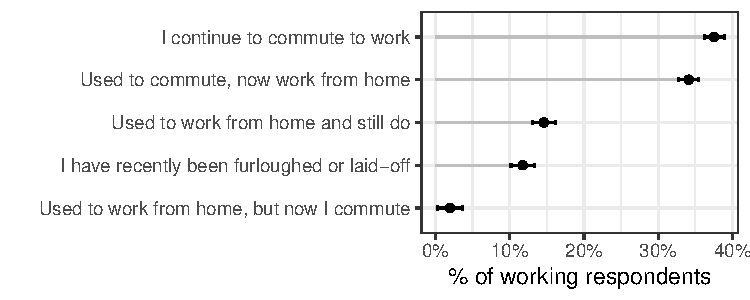
\includegraphics[width = \linewidth]{plots/working_summary.pdf} \\
  \begin{footnotesize}
    \begin{singlespace}
      \emph{Notes:} Standard errors are reported. 
    \end{singlespace}
    \end{footnotesize}
\end{minipage}
\end{figure} 




\begin{figure}
  \caption{Answers to the question ``Have you started to work from home in the last 4 weeks?'', conditional upon being in the labor force from a US sample} \label{fig:gender}
\centering
\begin{minipage}{1.0 \linewidth}
  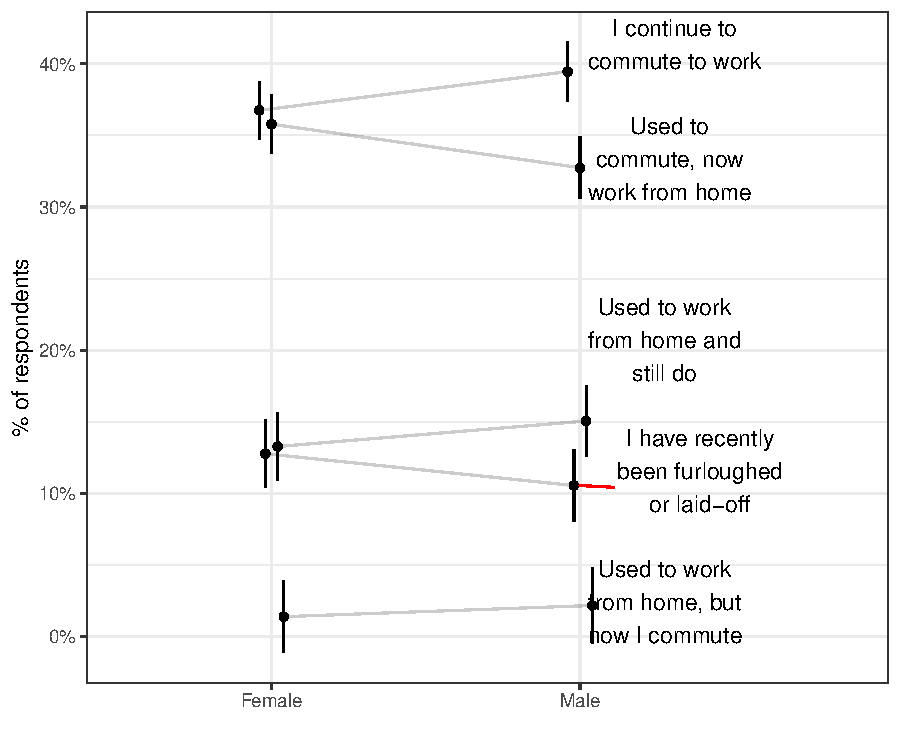
\includegraphics[width = \linewidth]{plots/gender.pdf} \\
  \begin{footnotesize}
    \begin{singlespace}
      \emph{Notes:} Standard errors are reported. 
    \end{singlespace}
    \end{footnotesize}
\end{minipage}
\end{figure} 



\newpage \clearpage
\bibliographystyle{aer}
\bibliography{remote_work.bib}

\end{document} 
